\documentclass{beamer}
\mode<presentation>
\usepackage{amsmath,amssymb}
\usepackage{color}
\usepackage{etoolbox}
\usepackage[dutch]{babel}
\usepackage{graphicx}
\usepackage{mathtools}
\usetheme{Rochester}
\usecolortheme{beaver}
\setbeamertemplate{footline}{\insertframenumber/\inserttotalframenumber}

%\setbeamercolor{normal text}{bg=black,fg=white}
%\setbeamercolor{frametitle}{bg=black,fg=white}
%\setbeamercolor{alerted text}{bg=black,fg=white}
%\setbeamercolor{title}{bg=black,fg=white}
%\setbeamercolor{stelling}{bg=black,fg=white}

\title{Adaptieve benaderingsmethodes}
\author{Jan Westerdiep}

\newcommand{\R}{\mathbb{R}}
\newcommand{\N}{\mathbb{N}}
\newcommand{\Z}{\mathbb{Z}}
\newcommand{\C}{\mathbb{C}}
\newcommand{\A}{\mathbb{A}}
\newcommand{\Q}{\mathbb{Q}}
\newcommand{\F}{\mathbb{F}}
\newcommand{\f}{\varphi}
\newcommand{\e}{\varepsilon}
\renewcommand{\d}{\delta}

\newtheorem{bewijs}{Bewijs}
\newtheorem{voorbeeld}{Voorbeeld}
\newtheorem{stelling}{Stelling}
\newtheorem{definitie}{Definitie}
\newtheorem{gevolg}{Gevolg}
\newtheorem{opmerking}{Opmerking}

\setbeamerfont{block title}{size=\small}

\begin{document}

\begin{frame}
\titlepage
\end{frame}

\begin{frame}{Wat?}
\begin{itemize}
  \item \alert<3>{Adaptieve} \alert<2>{benaderingsmethodes} \pause
  \item Functies benaderen \pause
  \item Door te kijken \emph{waar} de functie moeilijk is en daar in te zoomen \pause
  \item Dit alles aan de hand van twee artikelen van Peter Binev
\end{itemize}
\end{frame}

\begin{frame}{Iets preciezer}
\begin{columns}[t]
\begin{column}[T]{\linewidth - 2.5cm}
\begin{itemize}
  \item Pak $f: [0,1] \to \R$ met een partitie $P$ van $[0,1]$
  \uncover<2->{\item Pak beste stuksgewijs polynomiale benadering}
  \uncover<3->{\item Verfijn partitie d\'a\'ar waar beste benadering te slecht is}
  \uncover<4->{\item Herhaal}
\end{itemize}
\end{column}
\begin{column}[T]{2.5cm}
  \centering
  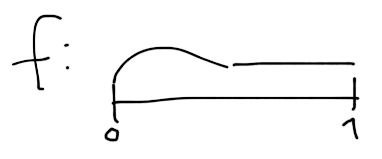
\includegraphics[width=\linewidth]{schets_0.png}\\
  \uncover<2->{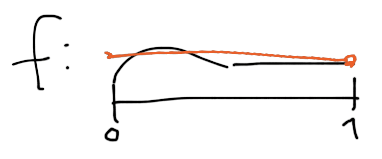
\includegraphics[width=\linewidth]{schets_1.png}\\}
  \uncover<3->{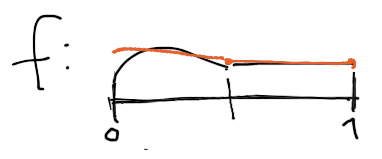
\includegraphics[width=\linewidth]{schets_2.png}\\}
  \uncover<4->{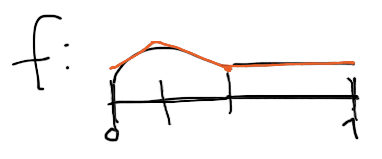
\includegraphics[width=\linewidth]{schets_3.png}\\}
\end{column}
\end{columns}
\end{frame}

\begin{frame}{Bij wie?}
  \begin{columns}[t]
    \begin{column}[T]{\linewidth - 2.5cm}
      Rob Stevenson
      \begin{itemize}
        \item Numerieke Analyse
        \uncover<2->{\item $\{$Research interests$\}$ $\ni$ adaptive approximation}
      \end{itemize}
    \end{column}
    \begin{column}[T]{2.5cm}
      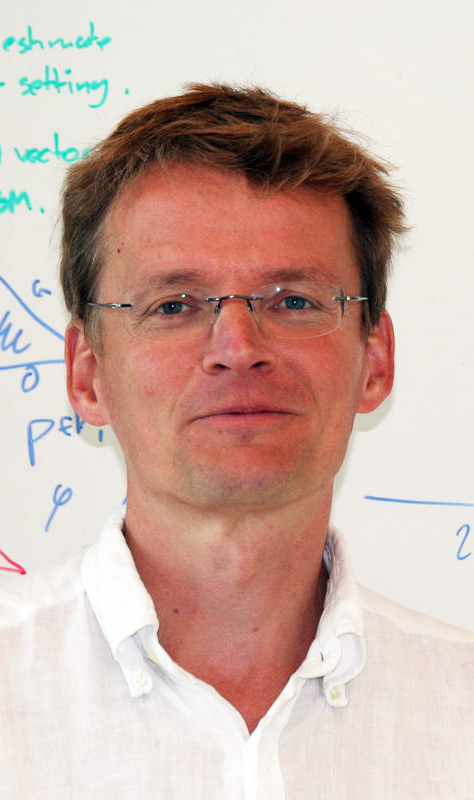
\includegraphics[width=2.5cm]{Stevenson_RP.jpg}
    \end{column}
  \end{columns}
\end{frame}

\begin{frame}{Waarom?}
  \begin{itemize}
    \item Wiskunde op de computer: goede samenkomst wiskunde/informatica \pause
    \item Spiksplinternieuw (2013) \pause
    \item Vraagstelling is makkelijk, de theorie erachter niet \pause
    \item Veel uitbreiding en toepassing mogelijk
  \end{itemize}
\end{frame}

\begin{frame}{Wanneer?}
  \begin{itemize}
    \item Februari, maart: Theorie begrijpen en opschrijven \pause
    \item Begin april: Implementeren in Python \pause
    \item April, mei: High Performance versie in C \pause
    \item Daarna: uitbreiding en toepassing bekijken
  \end{itemize}
\end{frame}

\begin{frame}{Adaptieve benaderingsmethodes}
  \centering
  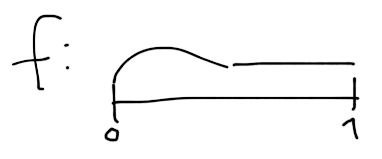
\includegraphics[height=1.7cm]{schets_0.png}\\
  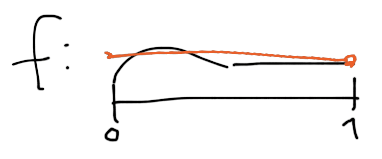
\includegraphics[height=1.7cm]{schets_1.png}\\
  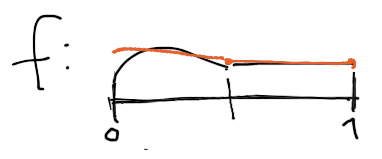
\includegraphics[height=1.7cm]{schets_2.png}\\
  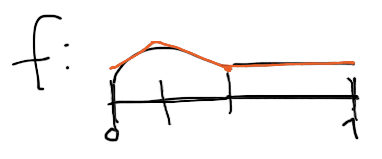
\includegraphics[height=1.7cm]{schets_3.png}\\
\end{frame}

\end{document}
